\section{Introduction}
\label{s:intro}


% In contrast, the broader robotics community can address very complex tasks; the robotic systems utilize many sensor modalities to build a coherent understanding of their environment.
% %
% By providing tested models of commercially available hardware, ROS/Gazebo provides a platform to study high-level behaviors while saving developer time during the design phase.  
% %
% Additionally, results have been shown to transfer to real robots, potentially addressing the ``reality-gap'' often encountered in ER~\cite{Koos2010}.  

% In the {\project} project, we have developed an evolutionary framework that integrates ROS-based simulations for robot evaluation.  
% %
% Our current prototype includes ROS, Gazebo, Ardupilot and MAVROS.    
% %
% The primary goals of the project are twofold. 
% %
% First, the framework enables researchers in ER to take advantage ROS and related simulation tools.
% %
% Second, it enables robot developers to employ evolutionary search during the design process.
% \pkm{I went back and pulled in some of the text from our original intro -- I think it still applies even with the 
% retooling to an Evo-ROS paper...}
%%%%%%%%%%%%%%%%%%%%%%%%%%%%%%%%%%%%
Mobile robotic systems are increasingly being deployed in a wide variety of
applications, such as public safety, agriculture, manufacturing, and supply chain. 
%
Traditionally such systems were operated by remote control, however,
advances in machine learning technologies are making it possible to build robots
that are either partially or fully autonomous.  
%
Such systems are often required to operate
in the face of uncertainty:
e.g., noisy communication, poor weather,
unexpected human input, faulty or damaged sensors and actuators.
% and dynamically adapt to, and
% even mitigate, those situations.
To successfully complete tasks despite adverse events and conditions,
systems must adapt to those situations.
%  requires designing systems that a coupling between system control software and 
% the hardware sensors and actuators that might experience partial or total failure.
% Whereas software and control algorithms can switch operating
% modes quite easily, many aspects of the hardware (for example, the placement 
% of sensors) are generally fixed by the time of deployment.
How can we design the physical robot and its control software so that 
it can operate effectively in such environments? 
The solution space for this problem is enormous, making exhaustive search impractical.

% Designing such systems is a challenging endeavor, one that can potentially be complemented by incorporating evolutionary search methods~\cite{Floreano2008}.  
%
The field of evolutionary robotics~(ER)~\cite{Floreano2008} attempts to address this challenging problem
%
by harnessing the open-ended search capabilities of evolutionary algorithms.
% simulation, many solutions can be explored identifying novel behaviors for different platforms~\cite{Cully2013}. 
An artificial genome specifies the robot's control system and possibly aspects of its morphology.
%
Individuals in a population are evaluated with respect to one or more tasks, with the best performing individuals selected to pass their genes to the next generation.
%
Evolutionary approaches have yielded effective controllers and physical designs for a variety of crawling, swimming, and flying robots~\cite{bongard-lipson, Lipson2000}.  
%
Our own research has applied evolutionary algorithms to optimize both morphology and control
in aquatic and terrestrial robots~\cite{Clark.JournalBB.2015,MooreALIFEJournal}.  
%
%Evolving robot behavior and morphology is interesting in its own right, but f
From an
engineering perspective, a major advantage of evolutionary search is the possible discovery of solutions (as well as potential problems) that the engineer might not otherwise have considered.

%%%%%%%%%%%%%%%%%%%%%%%%%%%%%%%%%%%% 
% 
%%%%%%%%%%%%%%%%%%%%%%%%%%%%%%%%%%%% 
Simulation is an essential component of ER, greatly reducing the time to evolve solutions while avoiding possible damage to physical robots.
%
The ER community typically creates one-off simulation environments by selecting from a few different physics 
engines~(e.g., ODE, Bullet, VoxCAD, Simulink, DART) to evaluate a candidate solution.  
%
Environments are sparse, generally featuring the robot and possibly a few obstacles.  
%
Tasks typically comprise locomotion, navigation, and basic problem solving.
%
% For example, Clark et. al.~\cite{Clark.ALIFE.2012} evolved a flexible caudal fin for a robotic fish using evolutionary search coupled with a physics simulation environment. 
%
% The simulator was customized for the specific problem, and would require a large programmer effort to retool for other problems.  
%
Robots themselves contain only a few sensors, most often custom developed for the specific 
experiment being conducted.  
%
Hence, ER tasks are often limited by the scope of the simulation environment and how much time a developer has to code obstacles, sensors, and the platform itself.  
%
Models are not necessarily shareable between developers due to a lack of standardization.  
%
While many research questions can, and have, been answered by simple simulations, 
it becomes difficult to address more complex questions in these environments.  
%%%%%%%%%%%%%%%%%%%%%%%%%%%%%%%%%%%% 

%%%%%%%%%%%%%%%%%%%%%%%%%%%%%%%%%%%%
In contrast, the broader robotics community can address very complicated tasks,
utilizing multiple sensors and actuators to interpret and navigate 
complex and often adverse environments.
% 
The Robot Operating System~(ROS)~\cite{ROS.main} was developed to facilitate reuse of control software 
across projects, and it has gained a large following in recent years.
%
Together with the Gazebo physics simulator~\cite{Gazebo_paper_ref}, these tools provide tested models of commercially available hardware, enabling study of high-level behaviors while saving developer time during the design phase. 
% The Robot Operating System~(ROS)~\cite{ROS.main} was developed to facilitate code reuse across projects.  
%
% Together with the Gazebo physics simulator~\cite{Gazebo.main}, they provide tested models of commercially available sensors and actuators.  
%
% Gazebo supports a wide variety of commercial sensors and actuators, while providing a robust, tested physics simulation environment for a wide variety of robotic platforms. 
%
% ROS/Gazebo thus provides a platform to study high-level behaviors while saving developer time during the design phase.  
%
Our early experiments~\cite{ClarkSSCI2017} demonstrated the potential benefits of integrating ROS/Gazebo with evolutionary search, but the customized nature of the simulation environment illustrated the need for a more
general platform.
%There, the Adabot uses pre-built, tested libraries for PID control, localization, and commercially available sensors.  
%
%Moreover, ROS control software readily transfers to a physical device.  
% Our early experiments using the Adabot platform~\cite{ClarkSSCI2017} highlight some benefits of integrating ROS/Gazebo with evolutionary search.  
%
%There, the Adabot uses pre-built, tested libraries for PID control, localization, and commercially available sensors.  %
% Still, the simulation environment was highly customized to a particular robotic platform,  illustrating  

%%%%%%%%%%%%%%%%%%%%%%%%%%%%%%%%%%%%

\begin{figure*}[!htb]
    \centering
    
    \begin{subfigure}[t]{0.33\textwidth}
        \centering
        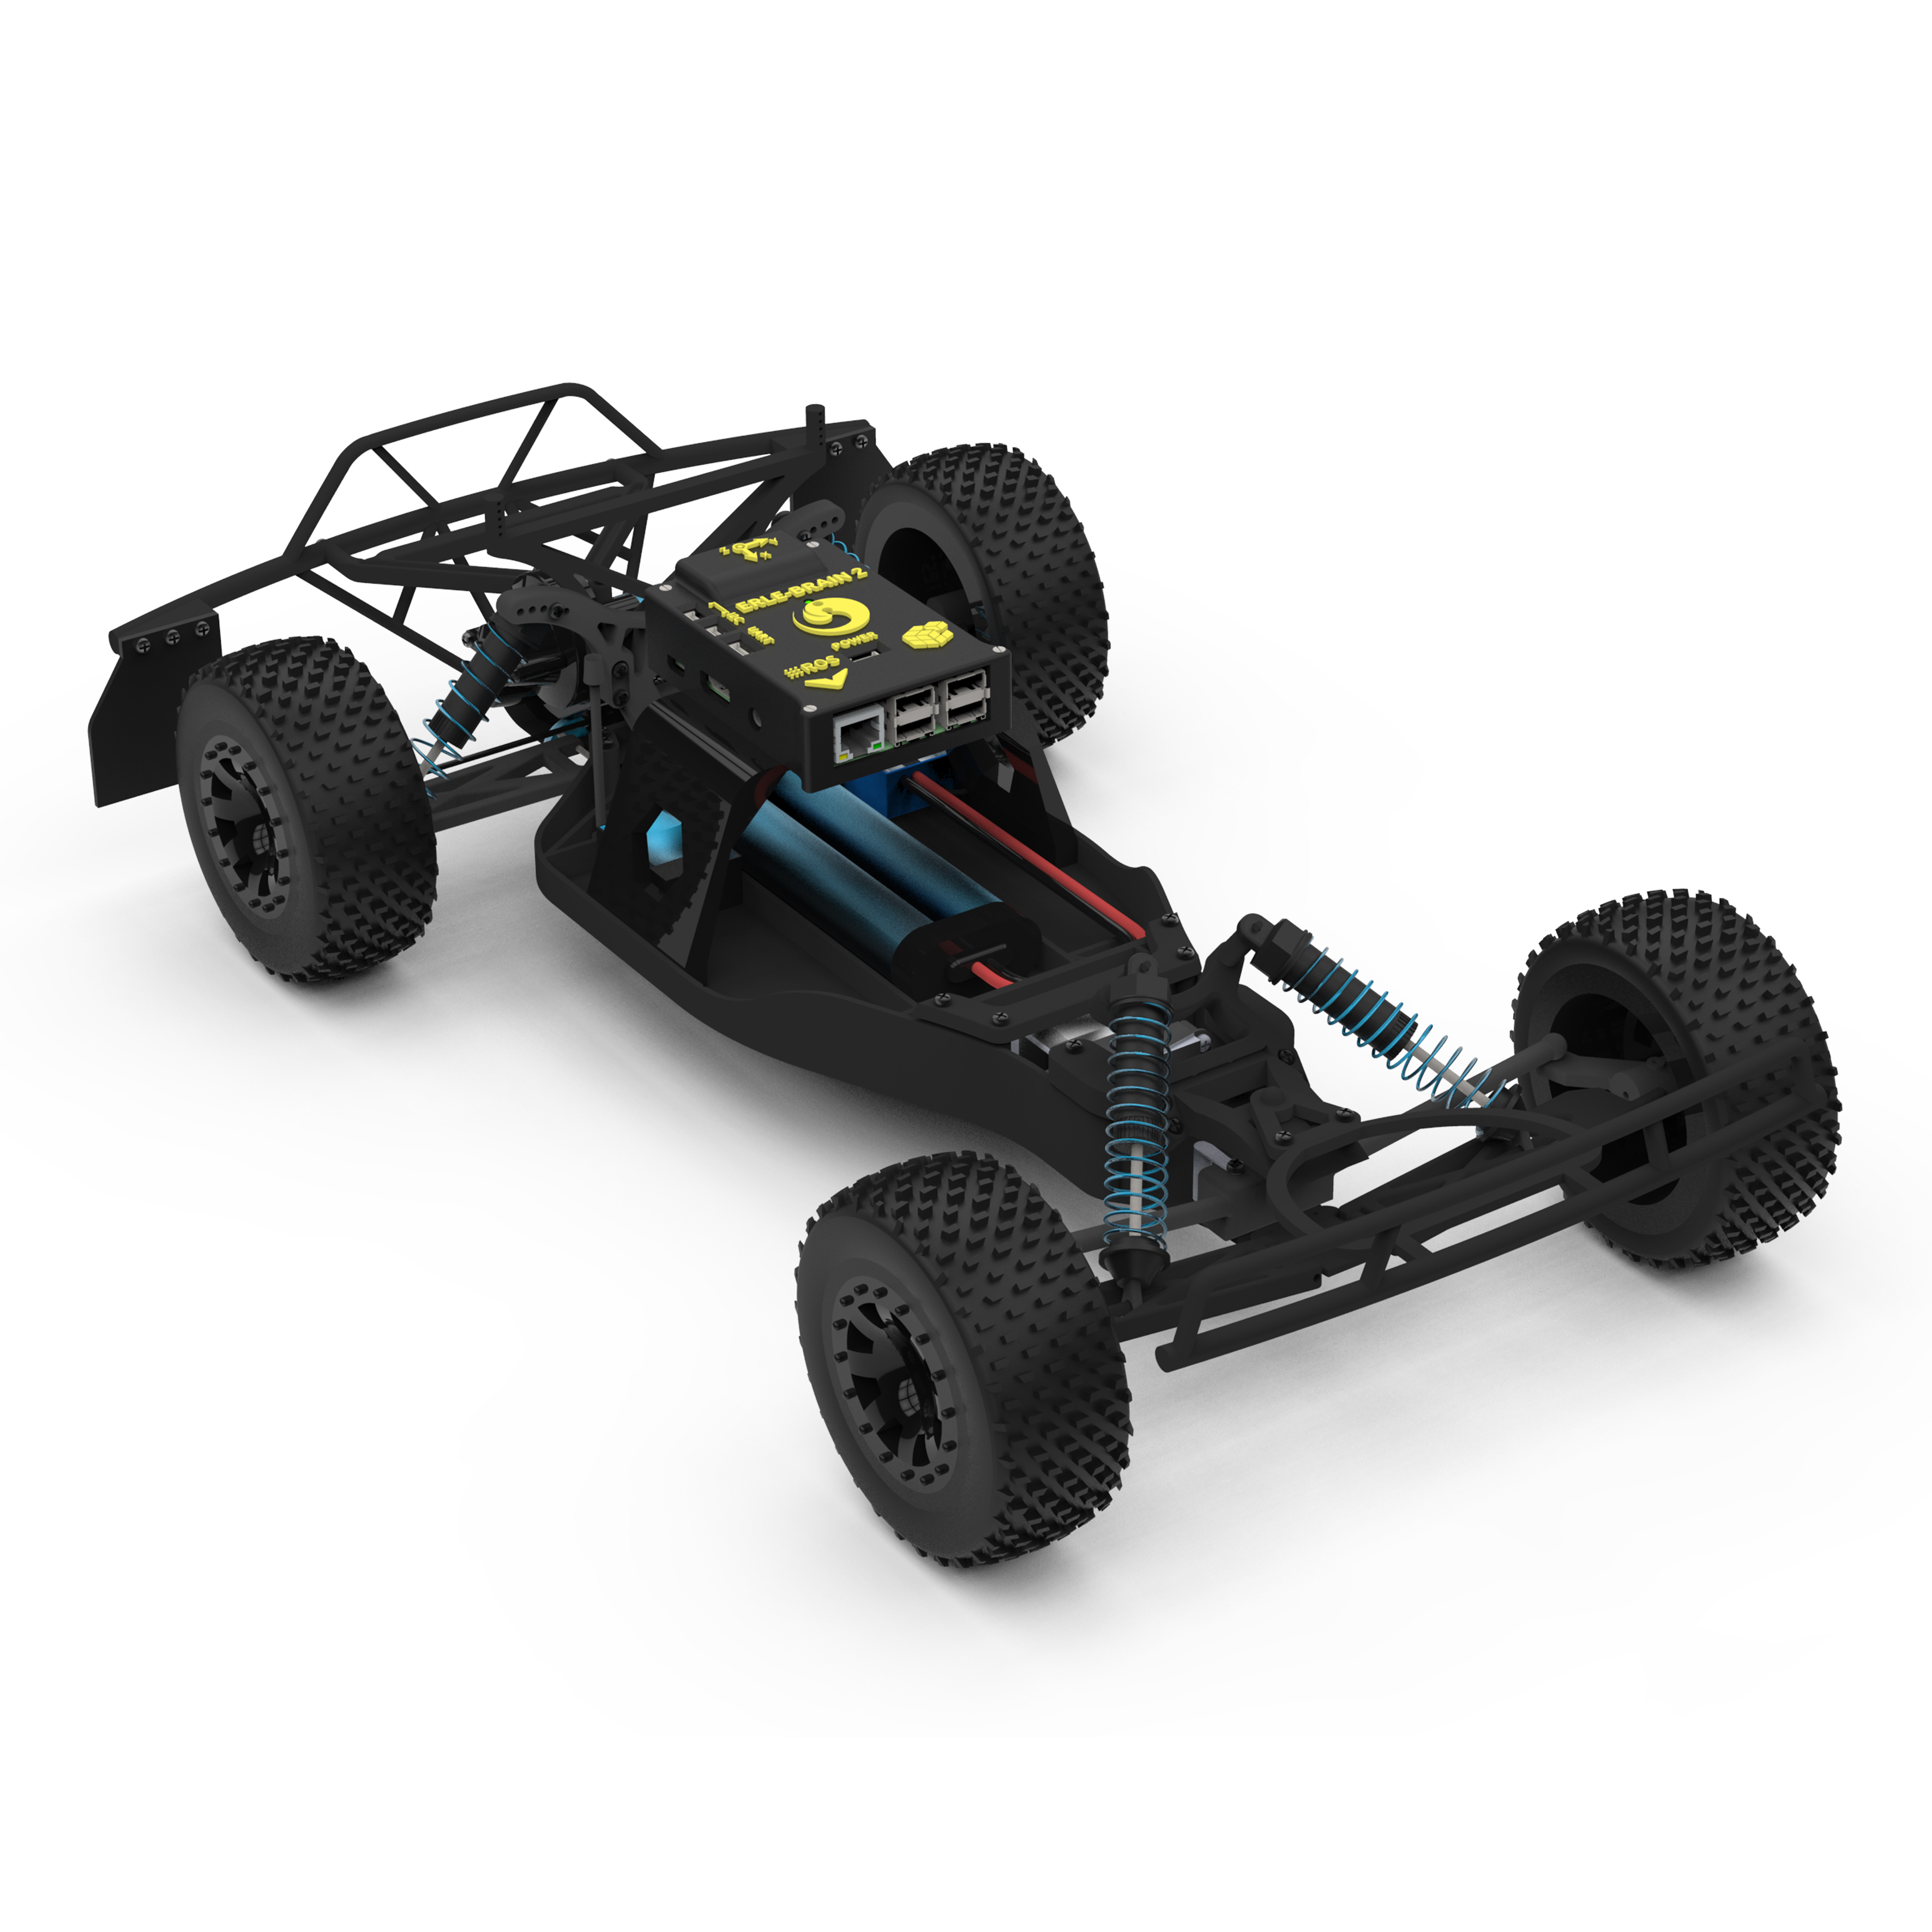
\includegraphics[height=1.2in]{Figures/ErleRover.jpg}
        \caption{Physical Erle-Rover frame}
        \label{real_rover}
    \end{subfigure}%
    ~ 
    \begin{subfigure}[t]{0.33\textwidth}
        \centering
        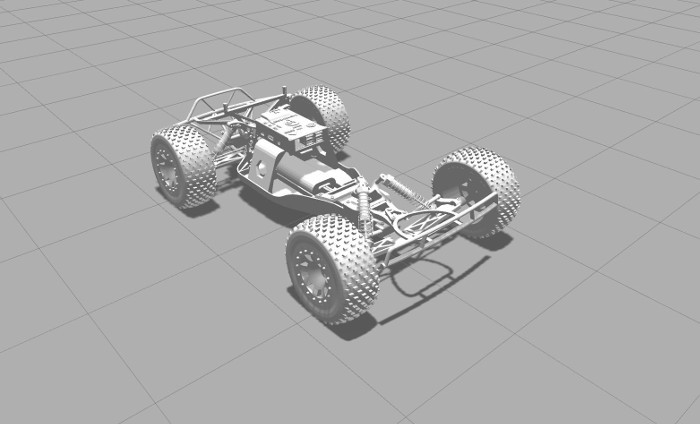
\includegraphics[height=1.2in]{Figures/rover.jpg}
        \caption{Gazebo simulated Erle-Rover}
        \label{sim_rover}
    \end{subfigure}
    ~
     \begin{subfigure}[t]{0.33\textwidth}
        \centering
        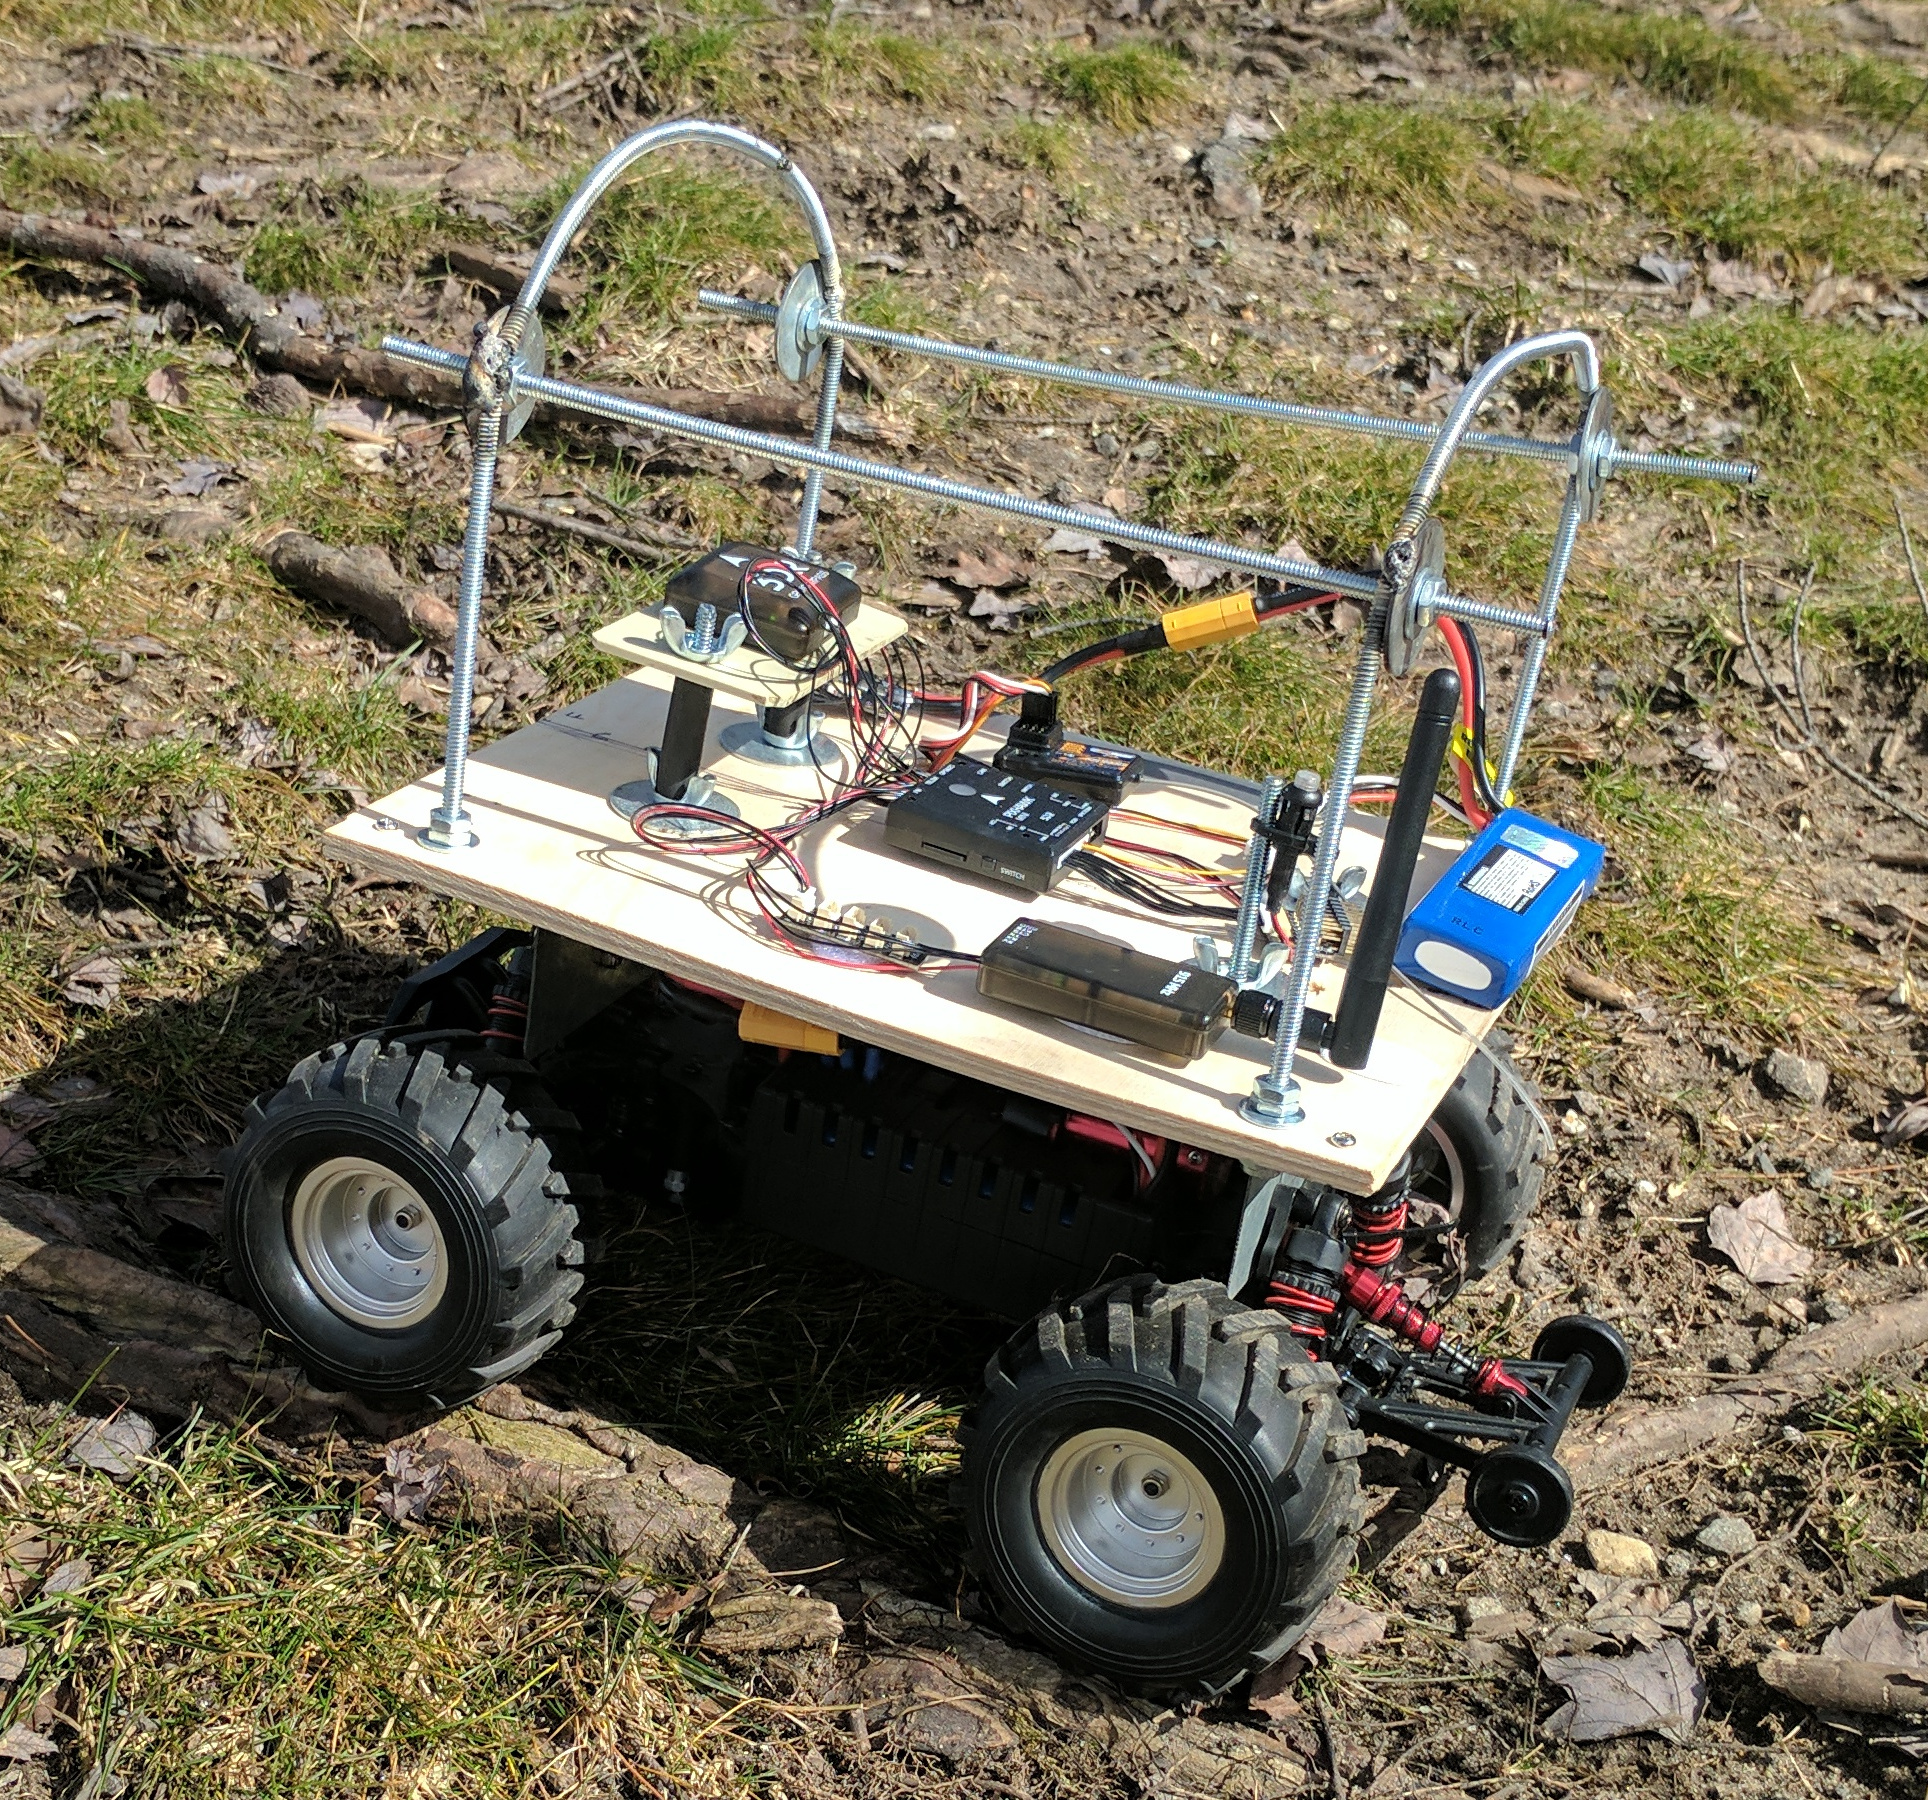
\includegraphics[height=1.2in]{Figures/real_rover_cropped.jpg}
        \caption{Physical rover frame equipped with sensor board, sensors, and a roll cage}
        \vspace{-0.1in}
        \label{msu_rover}
    \end{subfigure}
    \caption{The unmanned ground vehicle platform used in this study.}
    \label{rover_pics}
    \vspace{-0.12in}
\end{figure*}

%%%%%%%%%%%%%%%%%%%%%%%%%%%%%%%%%%%%
The main contribution of this paper is to 
describe Evo-ROS, a software framework integrating evolutionary search, ROS, and Gazebo.  
The current design provides a genetic-algorithm front-end and 
distributes evaluations across many ROS/Gazebo worker instances.  
To our knowledge Evo-ROS is the first ER system that includes simulation tools regularly employed by the broader robotics community.
%
% and available at \url{https://github.com/gsimon2/ros_catkin_ws_src/tree/master/evo_ros}.  
%
%
Evo-ROS internals are described in Section~\ref{s:evoros}. 
Evo-ROS is open-source; a \url{github} link is available at the end of the paper.
%
To demonstrate the operation of Evo-ROS, we conducted a case
study to optimize the 
placement and configuration of sonar sensors on unmanned ground vehicles (UGVs) that may
experience random sensor failures and loss of multiple sensors
due to physical damage.
The target platform is the Erle-Rover~\cite{erle.rover.main}, a commercial terrestrial robot which we 
have tasked with waypoint following under sensor uncertainty. 
%
Figure~\ref{rover_pics} shows the Erle-Rover, its simulation model, and a physical rover equipped with additional sensors. 
Sections~\ref{s:rover} and~\ref{s:results}, respectively, describe the experiments and results of the case study.
%
%Our initial experiment also illuminates areas for ongoing development of the framework, which we discuss later.  
%%%%%%%%%%%%%%%%%%%%%%%%%%%%%%%%%%%%
% 
%%%%%%%%%%%%%%%%%%%%%%%%%%%%%%%%%%%%
% The contributions of this paper are as follows: 
%
% First, we describe the Evo-ROS framework, a software package integrating evolutionary methods with simulation tools regularly employed by the broader robotics community.  
%
%The main To the best of the authors' knowledge, Evo-ROS is the fithis is the first software package to do so.  
%
% Second, we demonstrate the use of Evo-ROS to help design more resilient autonomous systems.  
%
% Specifically, we apply evolution to determine the location of sonar sensors for waypoint following and obstacle avoidance in a commercial unmanned ground vehicle~(UGV), despite random sensor failures and physical damage affecting multiple sensors.  
% 
Finally, in Section~\ref{s:conclusions}, we identify areas for improvement by discussing issues that arose 
during the case study.
%%%%%%%%%%%%%%%%%%%%%%%%%%%%%%%%%%%%